\documentclass[12pt]{article} \usepackage{url, graphicx}

% page layout
\setlength{\topmargin}{-0.25in}
\setlength{\textheight}{9.5in}
\setlength{\headheight}{0in}
\setlength{\headsep}{0in}

% problem formatting
\newcommand{\problemname}{Problem}
\newcounter{problem}

% math
\newcommand{\dd}{\mathrm{d}}

% primary units
\newcommand{\rad}{\mathrm{rad}}
\newcommand{\kg}{\mathrm{kg}}
\newcommand{\m}{\mathrm{m}}
\newcommand{\s}{\mathrm{s}}

% secondary units
\renewcommand{\deg}{\mathrm{deg}}
\newcommand{\km}{\mathrm{km}}
\newcommand{\mi}{\mathrm{mi}}
\newcommand{\h}{\mathrm{h}}
\newcommand{\ns}{\mathrm{ns}}
\newcommand{\J}{\mathrm{J}}
\newcommand{\eV}{\mathrm{eV}}
\newcommand{\W}{\mathrm{W}}

% derived units
\newcommand{\mps}{\m\,\s^{-1}}
\newcommand{\mph}{\mi\,\h^{-1}}
\newcommand{\mpss}{\m\,\s^{-2}}

% random stuff
\sloppy\sloppypar\raggedbottom\frenchspacing\thispagestyle{empty}

\begin{document}

\noindent
Name: \rule[-1ex]{0.55\textwidth}{0.1pt}
NetID: \rule[-1ex]{0.2\textwidth}{0.1pt}

\section*{NYU Physics I---Term Exam 3}

\paragraph{\problemname~\theproblem:}\refstepcounter{problem}%
(from lecture 2017-10-10)
A soft rubber ball of mass $0.1\,\kg$ drops from a height of about
$1\,\m$ onto a concrete floor and bounces. What is the mean force on
the ball from the floor while it is contact with the floor? Imagine
that the ball is in contact with the floor for about $10^{-4}\,\s$. If
you need to assume anything else to solve the problem, state your
assumptions.

\vfill

\paragraph{\problemname~\theproblem:}\refstepcounter{problem}%
(from lecture 2017-10-17)
Without using a calculator, estimate the sine of the angle $0.05~\deg$.
Use the small-angle approximation! (\emph{Hint:} Degrees aren't radians.)

\vfill

\paragraph{\problemname~\theproblem:}\refstepcounter{problem}%
(from bouncing worksheet)
An elastic ball of mass $m$ heads at speed $v$ towards a huge wall.
Its initial velocity is at an angle of $\theta$ to the normal.
Imagine that the collision is perfectly elastic and the
wall is perfectly frictionless, so the ``angle of incidence equals the
angle of reflection''. What is the magnitude of the momentum change of the ball (final
minus initial)?
Give your answer in terms of the symbols in the diagram.
\marginpar{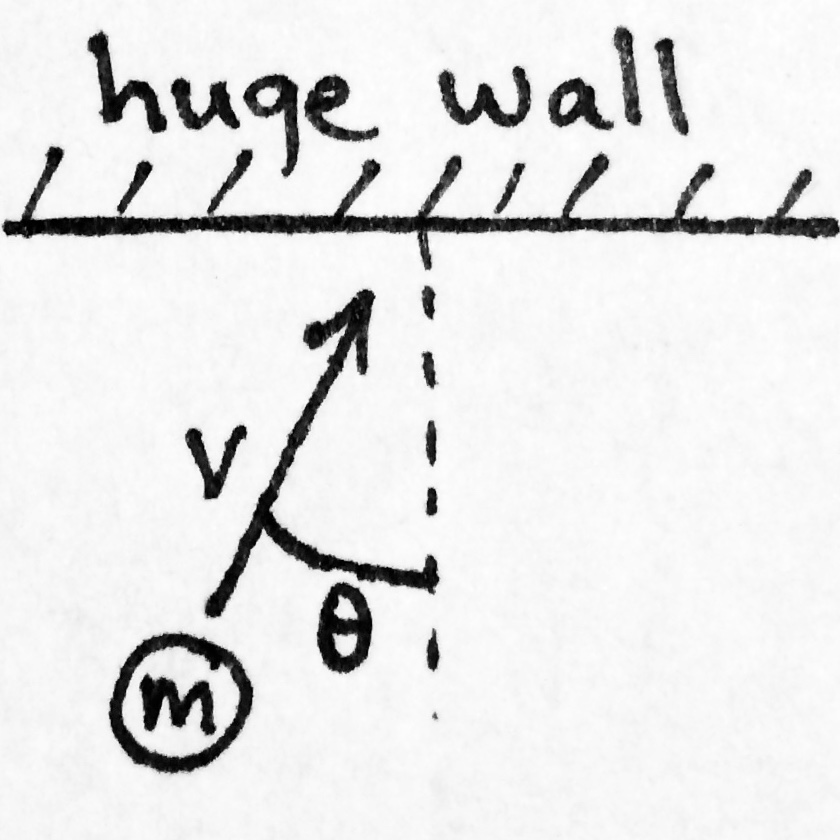
\includegraphics[width=1in]{../jpg/ballwall.jpg}}

\vfill
~
\clearpage
\paragraph{\problemname~\theproblem:}\refstepcounter{problem}%
(from Problem Set 5, problem 1) A small particle of mass $M$ and a small particle of mass
$m$ are separated by a distance $R$. How far is the center of mass of
the system from the center of the $M$ particle? Give your answer in terms of
$M$, $m$, and $R$. If you have to assume anything else to answer the
question, say what that is.

\vfill

\paragraph{\problemname~\theproblem:}\refstepcounter{problem}%
(from Problem Set 6, problem 3) A heavy package of $200\,\kg$ is
dragged $3\,\m$ horizontally across a surface by a horizontal
rope. The coefficient of sliding friction is $\mu = 0.2$. How much
heat is generated by this?  Assume $g = 10\,\mpss$, and give your
answer in Joules. If you need to assume anything else to solve this
problem, state it.

\vfill

\paragraph{\problemname~\theproblem:}\refstepcounter{problem}%
(from Problem Set 6, problem 4) Choose the pivot as the axis for
rotation, and counter-clockwise rotations or torques as positive
torques. What is the torque on the beam $m_\mathrm{b}$ from the cable $T_1$?
Give your answer in terms of the quantities given on the diagram.
\marginpar{\includegraphics[width=1in]{../mp/hanging_sign.pdf}}

\vfill
~
\end{document}
